\documentclass[a4paper,UKenglish,cleveref, autoref, thm-restate]{template/lipics-v2021}

\usepackage{float}
\usepackage[ruled]{algorithm2e}
\usepackage{adjustbox}
\usepackage[rightcaption]{sidecap}
\usepackage{proof}
\sidecaptionvpos{figure}{c}
\usepackage{todo}
\usepackage[toc,page]{appendix}
\usepackage{amsmath}
\usepackage{listings}
\usepackage{xcolor}
\usepackage{pgfplots}

\bibliographystyle{plainurl}

\newcommand{\hof}{HOF\xspace}
\newcommand{\hofs}{HOFs\xspace}
\newcommand{\lss}{LSS\xspace}
\newcommand{\cps}{CPS\xspace}
\newcommand{\stg}{STG\xspace}
\newcommand{\ghc}{GHC\xspace}
\newcommand{\sml}{SML\xspace}

\newcommand\catenate{\mathbin{\text{\ttfamily\upshape ++}}}

\definecolor{codegreen}{rgb}{0,0.6,0}
\definecolor{codegray}{rgb}{0.5,0.5,0.5}
\definecolor{codepurple}{rgb}{0.27, 0, 0.69}
\definecolor{backcolour}{rgb}{0.95,0.95,0.92}

\lstdefinestyle{mystyle}{
    backgroundcolor=\color{backcolour},   
    % commentstyle=\color{codegreen},
    % keywordstyle=\color{codepurple},
    % numberstyle=\tiny\color{codegray},
    % stringstyle=\color{codepurple},
    basicstyle=\ttfamily\footnotesize,
    breakatwhitespace=false,         
    breaklines=true,                 
    captionpos=b,                    
    keepspaces=true,                 
    numbers=left,                    
    numbersep=5pt,                  
    showspaces=false,                
    showstringspaces=false,
    showtabs=false,                  
    tabsize=2
}

\lstset{style=mystyle}


\title{Lambda Set Specialisation for Haskell}

\author{Sebastiaan Koppen}{Utrecht University, Netherlands}{}{}{}
\author{Hans Lous}{Utrecht University, Netherlands}{}{}{}
\author{Sem van Nieuwenhuizen}{Utrecht University, Netherlands}{}{}{}
\author{Martijn Voorwinden}{Utrecht University, Netherlands}{}{}{}
\authorrunning{S. Koppen, H.H. Lous, R.S. van Nieuwenhuizen, M.C.B. Voorwinden}

\date{March 2025}

\Copyright{Sebastiaan Koppen, Hans Lous, Sem van Nieuwenhuizen, and Martijn Voorwinden}

\ccsdesc[100]{Software and its engineering $\rightarrow$ Polymorphism; Procedures, functions and subroutines}
\keywords{defunctionalisation, monomorphisation, type systems}

\pgfplotsset{compat=1.16}

\begin{document}

\maketitle

\begin{abstract}
  Defunctionalisation is a program transformation technique that aims to eliminate higher-order functions. When applied successfully, it can enable better static analysis, compiler optimisations, and - by extension - runtime performance. Early studies of defunctionalisation contributed the basic \textit{monovariant} defunctionalisation, which is easily applied, but can suffer from an issue known as poisoning where the behaviour of a defunctionalised function is negatively affected by the introduction of new calls to that function. Specialising defunctionalisation methods mitigate this problem by tailoring the defunctionalisation procedure to specific calls, but they cannot always be applied. Brandon et al. introduced a new technique called lambda set specialisation. This is the first specialising defunctionalisation technique that does not restrict the way function values can be used. Our work extends their study with a translation from their research language, Morphic, to the popular functional language Haskell, allowing us to test the effects of lambda set specialisation while using \ghc. Like Brandon et al., we found an increase in performance, with a slight increase in binary size.
\end{abstract}

\section{Introduction}
Higher-order functions (\hofs) are a desirable and convenient feature found in many programming languages, particularly in functional programming. Programs making use of \hofs can be challenging to analyse - and thus also to optimise.

Many practical implementations rely on indirect jumps to heap-stored data, introducing a performance overhead. One widely used technique for addressing these issues is defunctionalisation, introduced by Reynolds \cite{reynolds1972definitional}, which transforms a program containing \hofs into a program containing only first-order functions.

Traditional defunctionalisation approaches replace \hofs with a single first-order function based on a finite set of representations of that function. While this method is simple to implement, it has a number of drawbacks - such as what is known as \textit{poisoning} \cite{wansbrough1999once}  (discussed in detail in section 2) - that much research has been dedicated to addressing. One idea that addresses some of these limitations is specialising defunctionalisation, where we may generate multiple first-order versions of a \hof based on its usage patterns. Many specialising defunctionalisation techniques impose some restrictions on how function values may be used or which \hofs can be defunctionalised.

Poisoning in this context means when a procedure that analyses properties of a program can get overwhelmed and fails to get accurate results. Examples can be call site analysis that fails to produce results when the program becomes too complex to analyse. In context of this paper we say a function poisons deinstitutionalisation techniques when these techniques fail to analyse the function and therefor have to fall back to dynamic dispatch. % expand or rewrite

Lambda Set Specialisation \cite{brandon2023better} (\lss), presents a novel approach to specialising defunctionalisation that does not impose any major restrictions. \lss operates within an extended type system, tracking function values and specialising them based on their usage context. It employs type inference, specialisation, and lowering passes to systematically replace \hofs with first-order counterparts while maintaining efficient compilation and analysis. The effectiveness of \lss has been demonstrated in the experimental functional language Morphic.

The Haskell functional programming language is to its core a lazy language. The most popular Haskell compiler is GHC, which uses the spineless tagless G-machine (STG) \cite{peyton1989spineless} as its lowest-level intermediate language. In this abstract machine \hofs are still present, which means that GHC does not include a defunctionalisation pass but implements \hofs with dynamic dispatch instead. The performance drawbacks of dynamic dispatch are mitigated by aggressive inlining performed during other compilation and optimisation passes. This makes Haskell an interesting case study for testing the effects of \lss.

In this work we will compare \lss with non-defunctionalising approach of GHC by leveraging a Morphic to Haskell translator to compare Haskell programs with and without \lss. Furthermore, we introduced a new benchmark to test the effect of \lss. We found that the haskell programs ran up to 1.26 times faster when compiling with \lss, with only a minor increase in binary size.

This paper is further organised as follows. In section 2 we describe the terms and techniques we employ. In section 3 we describe the translation of Morphic to Haskell in detail. Finally, the benchmarks and effects of \lss on Haskell are found in section 4 and 5 respectively.

\section{Preliminaries}\label{sec:preliminaries}

% Hans
In the most general sense, defunctionalisation refers to any program transformation that is semantics-preserving and which produces a transformed program without any higher-order functions. The transformation may not be total, that is, there may be programs that are impossible for the transformation to process. We identify two main types of defunctionalisation:
\begin{enumerate}[1.]
  \item \textit{monovariant} - where each \hof is transformed to at most one first-order function.
  \item \textit{specialising} - where a \hof may be transformed to more than one first-order function.
\end{enumerate}

The concept was first introduced by Reynolds \cite{reynolds1972definitional}, who presented a very simple approach for monovariant defunctionalisation. In Reynolds' approach, a \hof is replaced by a first-order function which - instead of a function parameter - takes a ``tag'' parameter. This tag represents a concrete function value with which the \hof is called. A special \texttt{apply} function is generated that dispatches to a function based on a tag parameter. Figure \ref{fig:ex-defunc} presents an example of this transformation. The \hof \texttt{map :: (a -> b) -> [a] -> [b]} is called with the \texttt{inc} and \texttt{double} functions, both of signature \texttt{Int -> Int}. After defunctionalisation, the signature of \texttt{map} becomes \texttt{Tag -> [Int] -> [Int]}, and its body makes use of the \texttt{apply :: Tag -> Int -> Int} function. This is a generated function that takes a tag parameter and dispatches to the corresponding closure.



\begin{figure}
  \centering
  \begin{minipage}[t]{0.45\textwidth}
    \begin{lstlisting}[language=Haskell]
inc    :: Int -> Int
double :: Int -> Int

map :: (a -> b) -> [a] -> [b]
map _ []       = []
map f (x : xs) = f x : map f xs\end{lstlisting}
  \end{minipage}
  \hfill
  \begin{minipage}[t]{0.53\textwidth}
    \begin{lstlisting}[language=Haskell]
map :: Tag -> [Int] -> [Int]
map _ []       = []
map t (x : xs) = apply t x : map t xs

apply :: Tag -> Int -> Int
apply Inc    x = inc x
apply Double x = double x\end{lstlisting}
  \end{minipage}
  \caption{Example of defunctionalising a program containing a single \hof \texttt{map} with two callsites. The left block shows the code as written, and the right block shows the defunctionalised code, with \texttt{map} a first-order function.}
  \label{fig:ex-defunc}
\end{figure}

Reynolds' very simple approach struggles with more complex higher-order programs, such as those containing \hofs that return a function. This restriction was addressed by later techniques such as the $\mathcal{A}$-algorithm of Chin et al. \cite{chin1996removal}. In addition, when applying Reynolds' transformation to polymorphic programs, it may produce transformed programs that -  although they are semantically equivalent to the source program - are impossible to type in the source language. The first total program transformation that could defunctionalise polymorphic higher-order programs to equivalent (and type-preserving) first order programs was presented by Bell et al. \cite{bell1997type} (by propagating type information), later Cejtin et al. \cite{cejtin2000flow} introduced an alternative approach based on control flow analysis. Another solution is to use generalied algebraic datatypes (GADTs) to define the tag datatype, as this allows us to add proper typing information to the tag constructors \cite{pottier2006polymorphic}.

Monovariant defunctionalisation techniques often suffer from a limitation known as \textit{poisoning}. In essence, since one \texttt{apply} function is generated for every callsite, one callsite of a \hof affects every other callsite. This can lead to unpredictable results for the programmer, as two callsites in completely unrelated parts of the codebase may affect each other. Figure \ref{fig:ex-poisoning} contains an example of this problem:
\texttt{map} has two callsites, one a very simple application of \texttt{map} to a single function \texttt{f}, and one where a choice between two functions \texttt{g} and \texttt{h} is made in an if-then-else. The first callsite could easily be inlined, but after defunctionalisation of the \texttt{map} function, this is no longer clear from the callsite: instead of \texttt{map f xs} the callsite now looks like \texttt{map TagF xs}, preventing the compiler from expanding the definition of \texttt{f}, analysing its function body and inlining it. So, we say that the second callsite has poisoned the first, preventing useful optimisations.

Specialising defunctionalisation approaches generally avoid the poisoning problem, and have other advantages such as avoiding large jump tables and enabling more aggressive optimisations of the less general \hof callsites downstream in the compilation process. Specialising defunctionalisation techniques tend to limit the ways in which \hofs can be used if we want to defunctionalise them. For instance, Rust \cite{klabnik2023rust} and C++ \cite{stroustrup2013cpp} both use a form of defunctionalisation in which \hofs are specialised to each callsite. This prevents poisoning, but in some more general cases of \hofs both languages revert to dynamic dispatch and indirect jumps. The array programming language Futhark also uses a form of specialising defunctionalisation, but limits the ways in which lambdas can be used at the type level, preventing functions from being full first-class citizens \cite{hovgaard2018higher}.

\begin{figure}
  \centering
  \begin{minipage}[t]{0.45\textwidth}
    \begin{lstlisting}[language=Haskell]
let f = \x -> x + 1 in
map f xs\end{lstlisting}
  \end{minipage}
  \hfill
  \begin{minipage}[t]{0.53\textwidth}
    \begin{lstlisting}[language=Haskell]
let g = \x -> x * x
    h = \x -> x + x
    func =
        if len(xs) > 10
        then g
        else h
    in
map func xs\end{lstlisting}
  \end{minipage}
  \caption{This figure shows two callsites of \texttt{map}. The left callsite is a very simple call to a \hof, that may be inlined at later compilation stages. The right callsite prevents this, however, since after monovariant defunctionalisation, map will have to accomodate all of \texttt{f}, \texttt{g}, and \texttt{h}. We say that the second callsite has `poisoned' the first. In this example we choose between two lambdas at the second callsite, which is a common example of where specialising defunctionalisation fails.}
  \label{fig:ex-poisoning}
\end{figure}

A recent paper by Brandon et al. \cite{brandon2023better} introduces a specialising defunctionalisation technique they call lambda set specialisation (\lss). The technique infers, for each \hof callsite, a set of lambdas with which the \hof can be called at that location. It then specialises first-order variants of the \hof for that callsite. A key innovation of the paper is that these lambda sets become part of the type of \hofs and that they can be polymorphic over this type, which then enables the use of well-known algorithms from type theory to infer the ``type'' of any call to the \hof. This type corresponds to the set of lambdas the \hof can be called with, this information is then used to produce specialised first-order versions of the \hof. The only restriction imposed by \lss is that any \hofs it defunctionalises must not be mutually recursive, which is much less restrictive than other specialising techniques. This makes \lss the first specialising defunctionalisation technique that does not impose any major restrictions on the use of function values.

To illustrate the result of using \lss to defunctionalise a program, see Figure \ref{fig:ex-lss}. Here, we defunctionalise the program from Figure \ref{fig:ex-poisoning} using \lss. In the intermediate, annotated program the \texttt{map} function now takes a function argument of type $a\stackrel\alpha\to b$, where $\alpha$ represents a set of possible function values (a lambda set). \texttt{map} then becomes polymorphic over $\alpha$ in the intermediate representation, with the callsites instantiating $\alpha$ to concrete lambda sets. In this case, the \texttt{map f xs} callsite calls $\texttt{map}\langle\{\texttt{f}\}\rangle$, since \texttt{f} is the only possible lambda value. Meanwhile, the \texttt{map func xs} callsite calls $\texttt{map}\langle\{\texttt{g,h}\}\rangle$ since both \texttt{g} and \texttt{h} are possible values for the lambda. During defunctionalisation, specialised versions of the \texttt{map} function are then generated
based on the lambda set annotations of the intermediate program. These specialised version are capable of handling complex control flow (like choosing between two lambdas in an if-then-else) while simultaneously allowing for the simple \texttt{map f xs} callsite to be further optimised.

\begin{figure}[ht]
  \centering
  \begin{align*}
    \text{Source program:}                  &                                                                                                                                             \\
    \texttt{map} :\quad                     & (a\to b) \to [a] \to [b]                                                                                                                    \\
    \text{call \texttt{map f}}:\quad        & \texttt{map f}                                                                                                                              \\
    \text{call \texttt{map func}}:\quad     & \texttt{map if len(xs) > 10 then g else h}                                                                                                  \\
    \\
    \text{Annotated program:}               &                                                                                                                                             \\
    \texttt{map}\langle\alpha\rangle :\quad & (a\stackrel\alpha\to b) \to [a] \to [b]                                                                                                     \\
    \text{call \texttt{map f}}:\quad        & \texttt{map}\langle\{\texttt{f}\}\rangle\ (\texttt{f as } (a\stackrel{\{\texttt{f}\}}{\to}  b))                                             \\
    \text{call \texttt{map func}}:\quad     & \texttt{map}\langle\{\texttt{g,h}\}\rangle\ (\texttt{(if len(xs) > 10 then g else h) as } (a\stackrel{\{\texttt{g}, \texttt{h}\}}{\to}  b)) \\
    \\
    \text{Defunctionalised program:}        &                                                                                                                                             \\
    \texttt{map1} :\quad                    & \texttt{TagF} \to [a] \to [b]                                                                                                               \\
    \texttt{map2} :\quad                    & \texttt{TagGH} \to [a] \to [b]                                                                                                              \\
    \text{call \texttt{map f}}:\quad        & \texttt{map1 F}                                                                                                                             \\
    \text{call \texttt{map func}}:\quad     & \texttt{map2 (if len(xs) > 10 then G else H)}
  \end{align*}
  \caption{An example of using LSS to defunctionalise the program from figure 2. The \texttt{map} function now takes a function argument of type $a \stackrel{\alpha}{\to} b$, where $\alpha$ represents a set of possible function values (a lambda set). \texttt{map} then becomes polymorphic over $\alpha$ in the intermediate representation, with the callsites instantiating $\alpha$ to concrete lambda sets. During defunctionalisation, we can then generate specialised version of the \texttt{map} function capable of handling complex control flow.}
  \label{fig:ex-lss}
\end{figure}

% monovariant v. specialising defunc.
% poisoning & expressiveness
% LSS

\section{Translation}\label{sec:trans}
This section describes the approach for translating Morphic programs to Haskell. The translation process aims to preserve the semantics of the original Morphic program as much as possible. This is not always possible due to the differences in evaluation strategy, handling of effects, and the difference in the order of instructions between the two languages. Due to our goals of evaluating \lss as a defunctionalisation technique for Haskell, we will only provide a one-way translation from Morphic to Haskell, and not the other way around.

In order to formally describe the translation process, we define a set of translation rules for the different constructs in Morphic. These rules are given in a natural deduction style, where the premises of the rule are the translations of the subexpressions of the construct, and the conclusion is the translation of the construct itself. In the rules the following syntax is used: $e \mapsto e'$, this denotes that the expression $e$ is translated to the expression $e'$.

The translation can largely be divided into three parts: the mapping of types between the two languages, the translation of language constructs, and the translation of built-in functions.

\subsection{Types}
The translation of types from Morphic to Haskell is based on the internal workings of the types used in the Morphic compiler, as well as the already existing translations from Morphic types to OCaml and \sml types by Brandon et al. \cite{brandon2023better}. Tuples, function types, and booleans map one on one to their Haskell counterparts. For a byte representation there were multiple choices, Morphic itself uses a number representation for bytes, while the translation to OCaml and \sml uses an ASCII character representation. We follow the Morphic representation and thus convert bytes to \verb|Word8| in Haskell. For integers we use \verb|Int64|, as morphic uses a 64 bit integer representation, while the size of a standard Haskell \verb|Int| is platform dependent. For floating point numbers we use \verb|Double|, as this is the same size as the floating point representation used in Morphic. For arrays, Morphic uses a persistent array implementation based on array mapped tries, which lines up with the \verb|Data.Vector.Persistent.Vector| \cite{Ravitch} implementation in Haskell. The translation rules for types can be seen in Figure \ref{fig:type-rules}.
\begin{figure}
  \centering
  \begin{gather*}
    \infer[\textsc{BoolType}]%
    {\textbf{Bool} \mapsto \textbf{Bool}}%
    {} \quad
    \infer[\textsc{ByteType}]%
    {\textbf{Byte} \mapsto \textbf{Word8}}%
    {} \\[1em]
    \infer[\textsc{IntType}]%
    {\textbf{Int} \mapsto \textbf{Int64}}%
    {} \quad
    \infer[\textsc{FloatType}]%
    {\textbf{Float} \mapsto \textbf{Double}}%
    {} \\[1em]
    \infer[\textsc{ArrayType}]%
    {\textbf{Array} \; \tau \mapsto \textbf{Data.Vector.Persistent.Vector} \; \tau'}%
    {\tau \mapsto \tau'} \\[1em]
    \infer[\textsc{TupleType}]%
    {(\tau_1,\dots,\tau_n) \mapsto (\tau_1',\dots,\tau_n')}%
    {\tau_1 \mapsto \tau_1' & \dots & \tau_n \mapsto \tau_n'} \quad
    \infer[\textsc{FuncType}]%
    {\tau_1 \mapsto \tau_2 \mapsto \tau_1' \mapsto \tau_2'}%
    {\tau_1 \mapsto \tau_1' & \tau_2 \mapsto \tau_2'}
  \end{gather*}
  \caption{Type translation rules.}
  \label{fig:type-rules}
\end{figure}

\subsection{Language Constructs and Built-in Functions}
The language constructs in Morphic line up well with those in Haskell. The main difference lies in the handling of side effects, as well as laziness. This affects the translation of function definitions, function calls, and let bindings. More on this can be found in the next section. Other constructs, such as case expressions and type definitions, can be directly translated to Haskell, as they only differ in syntax. The translation rules for language constructs can be seen in Figure \ref{fig:lang-rules}.

Built-in functions in Morphic are functions that are not part of the standard library, but are instead directly handled by the compiler. These functions are mainly used for input and output, as well as for array manipulation. They do not always have a direct counterpart in Haskell, but can be implemented using the standard library in conjunction with the \verb|persisent-vector| package \cite{Ravitch}. Formally, the relation between the inbuilt functions in Morphic and Haskell is defined by the translation rules in Figure \ref{fig:inbuilt-rules}.

Of the built-in functions, the \textbf{extract} function is the most complex to translate. This function takes an array and an index, and returns the element at that index, as well as a lamda expression that can be used to update the array at that index. This pattern allows for the caller to both read and write to the array, as if it were a mutable array. Since the \verb|Vector| type in Haskell does not provide a direct counterpart to this function, we translate it by combining existing functions from the \verb|persisten-vector| package.
\begin{figure}
  \centering
  \begin{gather*}
    \infer[\textsc{Call}]%
    {e_1 (e_2) \mapsto e_1' \; e_2'}%
    {e_1 \mapsto e_1' & e_2 \mapsto e_2'} \quad
    \infer[\textsc{ImpureCall}]%
    {\textbf{do } e_1 (e_2) \mapsto e_1' \; e_2'}%
    {e_1 \mapsto e_1' & e_2 \mapsto e_2'} \\[1em]
    \infer[\textsc{Func}]%
    {x(y_1: \tau_1,\dots,y_n: \tau_{n-1}): \tau_n = e \mapsto x :: \tau_1' \mapsto \dots \mapsto \tau_{n-1}' \mapsto \tau_n'\; ; \; x \; y_1 \dots y_n = e'}%
    {\tau_1 \mapsto \tau_1' & \dots & \tau_{n-1} \mapsto \tau_{n-1}' & \tau_n \mapsto \tau_n' & e \mapsto e'} \\[1em]
    \infer[\textsc{ImpureFunc}]%
    {\textbf{proc } e \mapsto e'}%
    {\textsc{Func } e \mapsto \textsc{Func } e'} \quad
    \infer[\textsc{Let}]%
    {\textbf{let } x = e_1 \textbf{ in } e_2 \mapsto \textbf{let } x = e_1' \textbf{ in seq } x \; e_2'}%
    {e_1 \mapsto e_1' & e_2 \mapsto e_2'} \\[1em]
    \infer[\textsc{Case}]%
    {\textbf{match } e_1 \{ e_2 \mapsto e_3,\dots,e_{n-1} \mapsto e_n\} \mapsto \textbf{case } e_1' \textbf{ of } e_2' \mapsto e_3';\dots;e_{n-1}' \mapsto e_n'}%
    {e_1 \mapsto e_1' & e_2 \mapsto e_2' & e_3 \mapsto e_3' & \dots & e_{n-1} \mapsto e_{n-1}' & e_n \mapsto e_n'} \\[1em]
    \infer[\textsc{TypeDef}]%
    {\textbf{type } x \{y_1 \tau_1,\dots,y_n \tau_n\} \mapsto \textbf{data } x = y_1 \tau_1' \; | \; \dots \; | \; y_n \tau_n'}%
    {\tau_1 \mapsto \tau_1' & \dots & \tau_n \mapsto \tau_n'} \\[1em]
    \infer[\textsc{Var}]%
    {x \mapsto x}%
    {x \in \text{Var}} \\[1em]
    \infer[\textsc{TrueConst}]%
    {\textbf{True} \mapsto \textbf{True}}%
    {} \quad
    \infer[\textsc{FalseConst}]%
    {\textbf{False} \mapsto \textbf{False}}%
    {} \\[1em]
    \infer[\textsc{ByteConst}]%
    {i\textbf{b} \mapsto i}%
    {i \in \mathbb{Z}_{\geq 0}} \quad
    \infer[\textsc{IntConst}]%
    {i \mapsto i}%
    {i \in \mathbb{Z}} \quad
    \infer[\textsc{FloatConst}]%
    {f \mapsto f}%
    {f \in \mathbb{R}} \\[1em]
    \infer[\textsc{ArrayConst}]%
    {[e_1,\dots,e_n] \mapsto \textbf{Data.Vector.Persistent.fromList} \; [e_1',\dots,e_n']}%
    {e_1 \mapsto e_1' & \dots & e_n \mapsto e_n'} \\[1em]
    \infer[\textsc{TupleConst}]%
    {(e_1,\dots,e_n) \mapsto (e_1',\dots,e_n')}%
    {e_1 \mapsto e_1' & \dots & e_n \mapsto e_n'} \\[1em]
  \end{gather*}
  \caption{Language construct translation rules.}
  \label{fig:lang-rules}
\end{figure}

\begin{figure}
  \centering
  \begin{gather*}
    \infer[\textsc{Output}]%
    {\textbf{output} (e) \mapsto \textbf{unsafePerformIO (putStrLn } e' )}%
    {e \mapsto e'} \\[1em]
    \infer[\textsc{Input}]%
    {\textbf{input} () \mapsto \textbf{unsafePerformIO getLine}}%
    {} \\[1em]
    \infer[\textsc{Panic}]%
    {\textbf{panic} (e) \mapsto \textbf{error } e'}%
    {e \mapsto e'} \\[1em]
    \infer[\textsc{Get}]%
    {\textbf{get} (e_1, e_2) \mapsto e_1'\; ! \; e_2'}%
    {e_1 \mapsto e_1' & e_2 \mapsto e_2'} \quad
    \infer[\textsc{Len}]%
    {\textbf{len} (e) \mapsto \textbf{length } e'}%
    {e \mapsto e'} \\[1em]
    \infer[\textsc{Push}]%
    {\textbf{push} (e_1, e_2) \mapsto \textbf{snoc } e_1' e_2'}%
    {e_1 \mapsto e_1' & e_2 \mapsto e_2'} \quad
    \infer[\textsc{Pop}]%
    {\textbf{pop} (e) \mapsto (\textbf{init } e', \textbf{last } e')}%
    {e \mapsto e'} \\[1em]
    \infer[\textsc{Extract}]%
    {\textbf{extract} (e_1, e_2) \mapsto (e_1' \; ! \; e_2', \backslash x \rightarrow e_1' \; // \; [e_2', x])}%
    {e_1 \mapsto e_1' & e_2 \mapsto e_2'}
  \end{gather*}
  \caption{Built-in function translation rules.}
  \label{fig:inbuilt-rules}
\end{figure}

\subsection{Non-preserved Semantics}
There are two areas where semantics are not fully preserved when translating Morphic to Haskell. The first area is the purity of functions. Due to a different approach to handling side effects in Morphic, impure function calls cannot be directly translated into Haskell without changing the order of instructions. Because of the difference in the order of intructions we do not preserve the purity of function, but instead circumvent it by using \verb|unsafePerformIO|. This may lead to optimisation issues downstream, but will not affect the correctness of the program, as the purity is correctly checked during the Morphic compilation. This loss of purity can be seen in the rules \textsc{ImpureCall} and \textsc{ImpureFunc} in Figure \ref{fig:lang-rules}, as well as in the rules \textsc{Output} and \textsc{Input} in Figure \ref{fig:inbuilt-rules}.

The second area is strictness; where Morphic is a strict language, Haskell is a lazy language. This means that the order of evaluation may differ between the two languages. Because of this, we force evaluate all local variables in the Haskell code through the use of \verb|seq|. This still differs from the Morphic semantics, where expressions are fully evaluated, whereas in Haskell, when using \verb|seq|, the expression is evaluated to weak head normal form. This should not affect the correctness of the program, as both languages being pure, thus the full evaluation of an expression should not have any side effects, outside of the use of the \verb|output| and \verb|input| functionsm which are correctly handled when using \verb|seq|. This affects the translation of let bindings, as can be seen in the rule \textsc{Let} in Figure \ref{fig:lang-rules}.
% Martijn

\section{Evaluation}
When evaluating \lss for Haskell, we seek to answer the following questions:
\begin{enumerate}
  \item How does \lss affect the performance of Haskell programs, as compared to the default behaviour of \ghc when compiling programs?
  \item How does \lss affect the binary size of Haskell programs, as compared to the default behaviour of \ghc when compiling programs?
\end{enumerate}
We seek to answer these questions to explore the potential benefits of \lss. The performance of programs is important, as it can affect the user experience of the program. The binary size of programs is important due to potential size restrictions on the target platform, this is especially important for embedded systems, where the size of the binary can be a limiting factor.

To answer the questions, we ran multiple benchmarks on Haskell programs compiled using \ghc\footnote{The benchmarking script and full results can be found at https://github.com/MartijnCBV/rmcs-bench-artifacts}, with and without \lss enabled by translating them from Morphic to Haskell\footnote{The adjusted Morphic compiler can be found at https://github.com/Ssoulner/morphic}.

\subsection{Benchmarking}\label{sec:bench}
\hofs have many practical applications, especially in functional programming languages to model things such as iteration and state. We wrote benchmarks in Morphic and used the existing benchmarks created by Brandon et al. \cite{brandon2023better}. These programs make use of \hofs in a number of different ways, mostly by including a function value in a data constructor. This makes any function that takes a parameter of that type or returns a value of that type a \hof. Our benchmarks use \hofs to implement the following things:
\begin{itemize}
  \item Iterators, by chaining and calling functions using the data type
        \begin{center}
          \verb|Iter(() -> Option (a, Iter a))|
        \end{center}
  \item Parsers, by chaining and calling functions using the data type
        \begin{center}
          \verb|Parse((Int, Array Byte) -> Option (Int, a))|
        \end{center}
  \item State, by chaining and calling functions using the data type
        \begin{center}
          \verb|State(s -> (s, r))|
        \end{center}
  \item A higher-order abstract syntax in an expression language, by incorporating values of type \verb|Expr -> Expr| in the expression language's data constructors.
\end{itemize}
The two largest benchmark programs are \verb|parse_json| and \verb|minhs|. The first makes extensive use of the parsing \hofs. The second also uses higher order parsing code and includes a higher order abstract syntax used for evaluating simple functional expressions.

\subsection{Experimental Setup}
To test the effects of \lss on Haskell code compiled using \ghc, the benchmark programs were translated into two Haskell programs per benchmark using the translator described in Section \ref{sec:trans}. The first program employs \lss, while the second program does not. Both programs were then compiled using \ghc version \verb|9.12.2| (the last stable version available at the time of writing this paper), with no optimisation flags (more on this can be found in the next section). After which the programs were run a hundred times each, on a machine with an \verb|Intel Core i9-14900HX CPU|, \verb|32GB 5600Mhz DDR5 RAM|, and running the Ubuntu 22 operating system through the windows subsystem for linux on Windows 11. Of these 100 runs, the minimum time taken, maximum time taken, mean time taken, median time taken, and standard deviation of the time taken were recorded. The results are shown and discussed in the next section. The complete data can be found in the extended results in Appendix \ref{sec:ext-res}.

\subsection{Results and Discussion}
Brandon et al. \cite{brandon2023better} found that \lss improved the performance of OCaml and \sml programs in most cases. They found that the binary size of the programs was reduced in certain cases due to downstream optimisations performing better on the code that was defunctionalised using \lss.

We found that the Haskell programs with \lss enabled were at least as fast as the Haskell programs without \lss enabled in all but one cases. With most benchmarks showing a speedup of 1.1 to 1.26 times. The MinHS benchmark, performed the worst, where \lss was resulted in a slowdown of 0.95 times. The relative speedup can be seen in Figure \ref{fig:performance}.

Furthermore, we found that the binary size of the Haskell programs with \lss enabled were bigger than the binary size of the Haskell programs without \lss enabled in all cases. This increase in binary sizes ranges from 1.01 times to 1.21 times. This is due to the fact that the defunctionalisation process increases the amount of functions in the program, which in turn increases the size of the binary. Due to the lack of further optimisations we do not see the same reduction in binary size due to downstream optimisations as Brandon et al. \cite{brandon2023better} found. The relative size of the binaries can be seen in Figure \ref{fig:binary}.

The results show that \lss can be beneficial for Haskell programs, when no further optimisations are used. The reason why we do not use further optimisations is due to a memory bug in the translated programs when compiling using the commonly used \verb|-o| and \verb|-o2| flags, which both enable a set of optimisations. We have not been able to diagnose what is causing this bug, but it might be due to the use of \verb|unsafePerformIO|, as this is known to cause issues with optimisations in Haskell. This is a limitation of our evaluation, as the results might be different if we were able to use these optimisations.

We can conclude that \lss can potentially be useful when included as a compiler pass in \ghc. For this reason, we recommend further research into the effects of \lss on Haskell programs, by implementing it as a \ghc plugin. Due to circumventing the translation of Morphic, it will be easier to diagnose potential memory issues, and enable further optimisations. This would show the true potential of \lss in the context of \ghc and allow for an evaluation to see if the same binary size reduction effect as observed by Brandon et al. \cite{brandon2023better} can be observed in Haskell programs compiled using \ghc.

Another avenue for further research is to investigate the effects of \lss on memory usage. Due to the increased amount of functions in the program, it is possible that the memory usage of the program increases. This could be a problem for programs that are memory constrained, and could potentially outweigh the benefits of the potential speedup that \lss provides.

\begin{figure}[htbp]
  \centering
  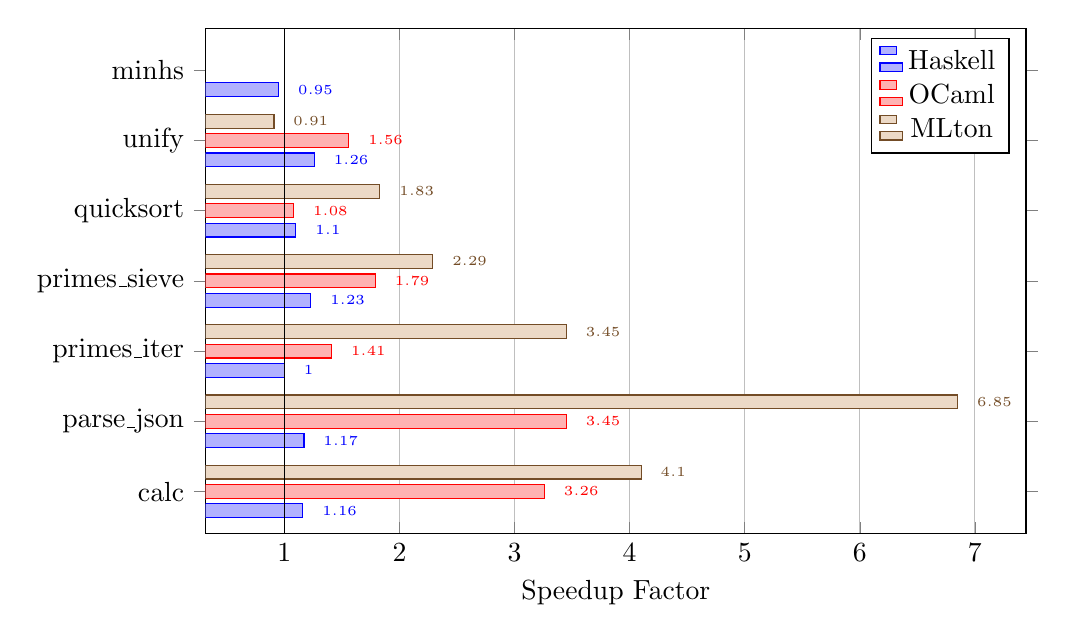
\begin{tikzpicture}
    \begin{axis}[
        % grid,
        xmajorgrids=true,
        xbar,
        symbolic y coords={calc, parse\_json, primes\_iter, primes\_sieve, quicksort, unify, minhs},
        bar width=5pt,
        enlarge y limits=0.1,
        nodes near coords,
        xlabel={Speedup Factor},
        % ylabel={Experiments},
        ytick=data,
        xtick={0,1,2,3,4,5,6,7},
        every node near coord/.append style={font=\tiny, xshift=3.5pt},
        width=12cm,
        height=8cm
      ]
      \addplot coordinates {(1.16,calc) (1.17,parse\_json) (1.00,primes\_iter) (1.23,primes\_sieve) (1.10,quicksort) (1.26,unify) (0.95,minhs)};
      \addplot coordinates {(3.26,calc) (3.45,parse\_json) (1.41,primes\_iter) (1.79,primes\_sieve) (1.08,quicksort) (1.56,unify)};
      \addplot coordinates {(4.1,calc) (6.85,parse\_json) (3.45,primes\_iter) (2.29,primes\_sieve) (1.83,quicksort) (0.91,unify)};
      \legend{Haskell, OCaml, MLton}
    \end{axis}

    \draw (1,0) -- (1,6.41cm);
  \end{tikzpicture}
  \caption{This figure shows the runtime speedup factor for each benchmark when compiled with LSS. Data for OCaml and MLton are taken from Brandon et al. \cite{brandon2023better}. For the Haskell results, the minimum runtime from 100 runs was used. The new benchmark \texttt{minhs} was only evaluated using Haskell.}
  \label{fig:performance}
\end{figure}

\begin{figure}[htbp]
  \centering
  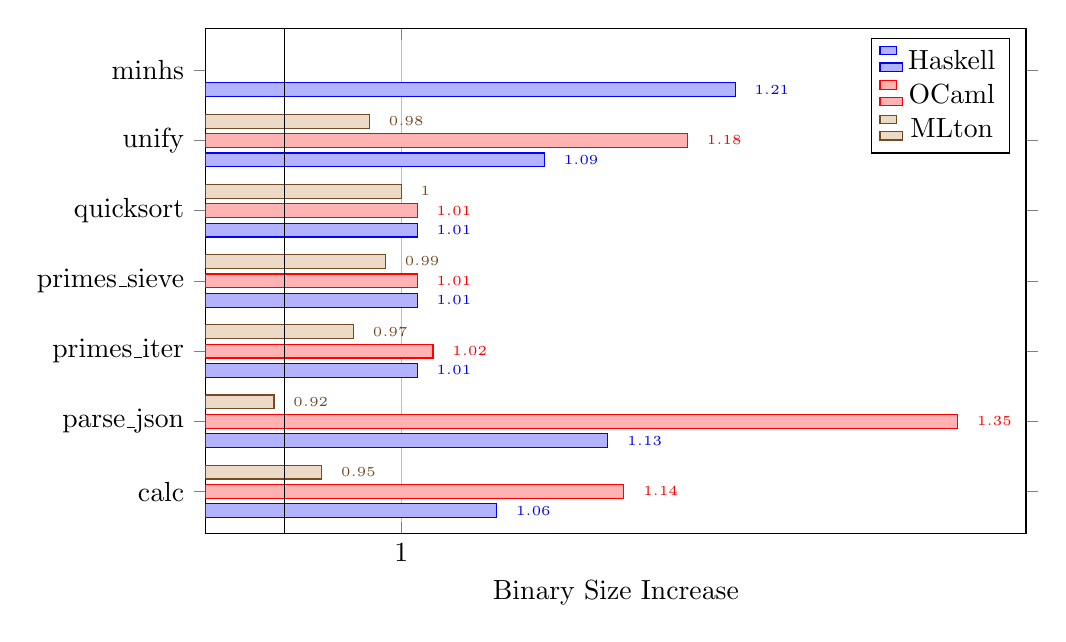
\begin{tikzpicture}
    \begin{axis}[
        % grid,
        xmajorgrids=true,
        xbar,
        symbolic y coords={calc, parse\_json, primes\_iter, primes\_sieve, quicksort, unify, minhs},
        bar width=5pt,
        enlarge y limits=0.1,
        nodes near coords,
        xlabel={Binary Size Increase},
        % ylabel={Experiments},
        ytick=data,
        xtick={0,1,2,3,4,5,6,7},
        every node near coord/.append style={font=\tiny, xshift=3.5pt},
        width=12cm,
        height=8cm
      ]
      \addplot coordinates {(1.06,calc) (1.13,parse\_json) (1.01,primes\_iter) (1.01,primes\_sieve) (1.01,quicksort) (1.09,unify) (1.21,minhs)};
      \addplot coordinates {(1.14,calc) (1.35,parse\_json) (1.02,primes\_iter) (1.01,primes\_sieve) (1.01,quicksort) (1.18,unify)};
      \addplot coordinates {(0.95,calc) (0.92,parse\_json) (0.97,primes\_iter) (0.99,primes\_sieve) (1.00,quicksort) (0.98,unify)};
      \legend{Haskell, OCaml, MLton}
    \end{axis}

    \draw (1,0) -- (1,6.41cm);
  \end{tikzpicture}
  \caption{This figure shows the relative binary size increase of benchmarks compiled with LSS and without LSS.}
  \label{fig:binary}
\end{figure}

% \begin{SCfigure}[][h]
%     
\includegraphics[width=0.75\textwidth]{Paper/speedup_chart.png}
%     \caption{Relative speedup of programs compiled with LSS enabled compared to compiling the programs without LSS enabled. For the comparison the minimum running time of a hundred runs was used.}
%     \label{fig:performance}
% \end{SCfigure}
% \begin{SCfigure}[][h]
%     \centering
%     
\includegraphics[width=0.75\textwidth]{Paper/bin_size_chart.png}
%     \caption{Relative size of binaries resulting from compiling programs with LSS enabled compared to compiling the programs without LSS enabled.}
%     \label{fig:binary}
% \end{SCfigure}

\section{Related Work}
Defunctionalisation and related techniques have been studied for decades. A first introduction to the generic monovariant defunctionalisation, was given in a seminal paper by Reynolds \cite{reynolds1972definitional}, with an algorithm to convert all calls to \hofs with calls to a single \texttt{apply} function, as was described in Section \ref{sec:preliminaries}.

An extension of this work was done by Minamide et al. \cite{minamide1996typed}, who showed that existential types, in combination with closure conversion, can be used to defunctionalise well-typed source languages to well-typed target languages. While compiler optimisations benefit from retaining this type information, the creation of closures can introduce runtime overhead. Cejtin et al. \cite{cejtin2000flow} show that this problem is limited in practice. They present a closure conversion algorithm that has limited compile-time overhead even for larger benchmarks.

A different approach is taken by Bell et al. \cite{bell1997type}, who identify challenges associated with applying defunctionalisation to polymorphic languages. Similar to monovariant defunctionalisation, they incorporate functional application types, enabling the defunctionalisation of polymorphic higher-order functions without the need for closures. Their approach builds on Reynolds' by introducing a method to translate well-typed source programs to well-typed target programs.

Fourtounis et al. \cite{fourtounis2014modular} introduce the concept of modular defunctionalisation, where different modules are defunctionalised separately and linked at a later stage of compilation. This method studies optimisations that are not directly related to specialisations, which could provide an opportunity to combine it with the lambda set specialisation from Brandon et al \cite{brandon2023better}.

Mitchell et al. \cite{mitchell2009losing} describes a concrete defunctionalisation method that works by repeatedly applying a set of rules on GHC's Core language. Their method is not integrated in the GHC compiler, but in the York Haskell Compiler \cite{golubovsky2007yhc}. Integrating LSS as a GHC compiler pass in a similar manner could provide a more realistic image of added benefit of LSS for Haskell.

Pottier et al. \cite{pottier2006polymorphic} introduces a monovariant defunctionalisation method that can handle polymorphic code. They abstractly analyse defunctionalisation and show that it is an instance of concretisation, which performs similar transformations on other constructs (such as records). They show how their method can be used to optimise compilation of Haskell's type classes.

Finally, Brandon et al. \cite{brandon2023better} introduced \lss and their language Morphic, which is the direct predecessor to this paper.



% Sebastiaan

\section{Conclusion}
% While defunctionalisation and continuation-passing style have been a research topic for several decades, we have yet to discover a \todo{"good" method(?)}


% Instead, the universally applicable monovariant defunctionalisation has been extended with a number of specialisations. An important discovery was the use of flow-analysis in guiding the defunctionalisation process, as it can be used to structure the case analysis corresponding to (higher-order) function calls. By extension, flow-analysis has proven useful for preserving types during defunctionalisation.

% While a number of specialising methods have been developed to optimise the defunctionalisation process in a specific context, we have yet to discover a unifying method. A large step in this direction was taken by Brandon et al. \cite{brandon2023better}, who make use of lambda set specialisation. This work extends on their research by introducing a translation method from Morphic to Haskell and comparing the runtime performence as well as the binary size of optimised (defunctionalised) and non-optimised programs. We found that LSS-specialisation can provide similar speedups as OCaml and \sml, with only a small increase in binary size.

While a number of defunctionalisation approaches have been developed, most of them lack in expressivity or suffer from poisoning. Brandon et al.\cite{brandon2023better} developed an approach which did not suffer from this. However, this approach is currently only available as a pass in the compiler for their language Morphic, and by extension for OCaml and SML through their respective backends in the Morphic compiler. We sought to extend on this result by implementing a Haskell backend for Morphic compiler to test if \lss would be worthwhile to implement in \ghc.

When benchmarking the resulting Haskell programs a speedup of up to 1.32x was found when employing \lss on some benchmarks, at the cost of increasing the binary size by up to 1.13x. Due to this it has the potential to be a useful extension to \ghc. For the newly introduced \texttt{minhs} benchmark, which is more complex than the other benchmarks, a slight decrease in performance was measured. Exploring the scalability of LSS would therefore be interesting for future work. However, to assess the capabilities of LSS in a more realistic setting, a promising approach would be to implement it as a compiler pass within GHC's Core language.




% Sebastiaan

\section*{Acknowledgments}
This work greatly benefited from the support of Benjamin Driscoll and William Brandon, who took the time to discuss their language (Morphic) and provided the inspiration for implementing and testing a parsing library benchmark.



\begin{appendices}

  \section{Extended Results}\label{sec:ext-res}
  This appendix contains the extended results of the benchmarks that were run for the evaluation of \lss for Haskell. The results consist of the minimum time taken, maximum time taken, mean time taken, median time taken, and standard deviation of the time taken out of a hundred runs for each benchmark.
  \begin{table}
    \begin{tabular}{l|c c}
      \textbf{calc}               & \textbf{Without LSS (sec)} & \textbf{With LSS (sec)} \\
      \hline
      \textbf{Minimum}            & 0.0710                     & 0.0610                  \\
      \textbf{Maximum}            & 0.0916                     & 0.0719                  \\
      \textbf{Mean}               & 0.0747                     & 0.0618                  \\
      \textbf{Median}             & 0.0714                     & 0.0614                  \\
      \textbf{Standard Deviation} & 0.0050                     & 0.0017                  \\
      \hline
      \textbf{minhs}              & \textbf{Without LSS (sec)} & \textbf{With LSS (sec)} \\
      \hline
      \textbf{Minimum}            & 0.5811                     & 0.6111                  \\
      \textbf{Maximum}            & 0.6113                     & 0.6612                  \\
      \textbf{Mean}               & 0.5878                     & 0.6231                  \\
      \textbf{Median}             & 0.5912                     & 0.6215                  \\
      \textbf{Standard Deviation} & 0.0063                     & 0.0074                  \\
      \hline
      \textbf{parse\_json}        & \textbf{Without LSS (sec)} & \textbf{With LSS (sec)} \\
      \hline
      \textbf{Minimum}            & 1.5488                     & 1.3193                  \\
      \textbf{Maximum}            & 1.7192                     & 1.4703                  \\
      \textbf{Mean}               & 1.5980                     & 1.3682                  \\
      \textbf{Median}             & 1.5888                     & 1.3602                  \\
      \textbf{Standard Deviation} & 0.0365                     & 0.0252                  \\
      \hline
      \textbf{primes\_iter}       & \textbf{Without LSS (sec)} & \textbf{With LSS (sec)} \\
      \hline
      \textbf{Minimum}            & 0.0209                     & 0.0208                  \\
      \textbf{Maximum}            & 0.0218                     & 0.0217                  \\
      \textbf{Mean}               & 0.0211                     & 0.0212                  \\
      \textbf{Median}             & 0.0211                     & 0.0212                  \\
      \textbf{Standard Deviation} & 0.0001                     & 0.0002                  \\
      \hline
      \textbf{primes\_sieve}      & \textbf{Without LSS (sec)} & \textbf{With LSS (sec)} \\
      \hline
      \textbf{Minimum}            & 0.2727                     & 0.2224                  \\
      \textbf{Maximum}            & 0.3131                     & 0.2931                  \\
      \textbf{Mean}               & 0.2849                     & 0.2360                  \\
      \textbf{Median}             & 0.2831                     & 0.2329                  \\
      \textbf{Standard Deviation} & 0.0082                     & 0.0098                  \\
      \hline
      \textbf{quicksort}          & \textbf{Without LSS (sec)} & \textbf{With LSS (sec)} \\
      \hline
      \textbf{Minimum}            & 1.0925                     & 0.9926                  \\
      \textbf{Maximum}            & 1.2533                     & 1.1129                  \\
      \textbf{Mean}               & 1.1423                     & 1.0397                  \\
      \textbf{Median}             & 1.1432                     & 1.0429                  \\
      \textbf{Standard Deviation} & 0.0237                     & 0.0199                  \\
      \hline
      \textbf{unify}              & \textbf{Without LSS (sec)} & \textbf{With LSS (sec)} \\
      \hline
      \textbf{Minimum}            & 1.4158                     & 1.1242                  \\
      \textbf{Maximum}            & 1.5658                     & 1.1952                  \\
      \textbf{Mean}               & 1.4829                     & 1.1559                  \\
      \textbf{Median}             & 1.4754                     & 1.1547                  \\
      \textbf{Standard Deviation} & 0.0391                     & 0.0148                  \\
    \end{tabular}
    \caption{Benchmark results comparing execution time with and without LSS optimisation}
  \end{table}

  \clearpage

\end{appendices}

\bibliography{main}


\newpage


\section*{AI Statement}
The use of AI for this paper has been limited to trivial questions such as \textit{1}. In this case, and most other cases where AI was consulted, its response was found to be incorrect. The AI provided an example similar to the one found in Appendix \ref{fig:ex-defunc}, but attempted to replace the function \texttt{map} itself by a data type, rather than the function value passed to it, resulting in a nonsensical example. This low quality output is likely due to the small amount of information available on this topic.

\noindent To summarise:
\begin{itemize}
  \item None of the content of this paper was directly generated by any form of AI, nor was any content based solely on the output of an AI.
  \item None of the code used and/or produced for this project was generated or modified by AI.
\end{itemize}

\end{document}
